% $Header$

\documentclass{beamer}

\usepackage{amsmath,amssymb,latexsym,eucal,amsthm,graphicx}
%%%%%%%%%%%%%%%%%%%%%%%%%%%%%%%%%%%%%%%%%%%%%
% Common Set Theory Constructs
%%%%%%%%%%%%%%%%%%%%%%%%%%%%%%%%%%%%%%%%%%%%%

\newcommand{\setof}[2]{\left\{ \, #1 \, \left| \, #2 \, \right.\right\}}
\newcommand{\lsetof}[2]{\left\{\left. \, #1 \, \right| \, #2 \,  \right\}}
\newcommand{\bigsetof}[2]{\bigl\{ \, #1 \, \bigm | \, #2 \,\bigr\}}
\newcommand{\Bigsetof}[2]{\Bigl\{ \, #1 \, \Bigm | \, #2 \,\Bigr\}}
\newcommand{\biggsetof}[2]{\biggl\{ \, #1 \, \biggm | \, #2 \,\biggr\}}
\newcommand{\Biggsetof}[2]{\Biggl\{ \, #1 \, \Biggm | \, #2 \,\Biggr\}}
\newcommand{\dotsetof}[2]{\left\{ \, #1 \, : \, #2 \, \right\}}
\newcommand{\bigdotsetof}[2]{\bigl\{ \, #1 \, : \, #2 \,\bigr\}}
\newcommand{\Bigdotsetof}[2]{\Bigl\{ \, #1 \, \Bigm : \, #2 \,\Bigr\}}
\newcommand{\biggdotsetof}[2]{\biggl\{ \, #1 \, \biggm : \, #2 \,\biggr\}}
\newcommand{\Biggdotsetof}[2]{\Biggl\{ \, #1 \, \Biggm : \, #2 \,\Biggr\}}
\newcommand{\sequence}[2]{\left\langle \, #1 \,\left| \, #2 \, \right. \right\rangle}
\newcommand{\lsequence}[2]{\left\langle\left. \, #1 \, \right| \,#2 \,  \right\rangle}
\newcommand{\bigsequence}[2]{\bigl\langle \,#1 \, \bigm | \, #2 \, \bigr\rangle}
\newcommand{\Bigsequence}[2]{\Bigl\langle \,#1 \, \Bigm | \, #2 \, \Bigr\rangle}
\newcommand{\biggsequence}[2]{\biggl\langle \,#1 \, \biggm | \, #2 \, \biggr\rangle}
\newcommand{\Biggsequence}[2]{\Biggl\langle \,#1 \, \Biggm | \, #2 \, \Biggr\rangle}
\newcommand{\singleton}[1]{\left\{#1\right\}}
\newcommand{\angles}[1]{\left\langle #1 \right\rangle}
\newcommand{\bigangles}[1]{\bigl\langle #1 \bigr\rangle}
\newcommand{\Bigangles}[1]{\Bigl\langle #1 \Bigr\rangle}
\newcommand{\biggangles}[1]{\biggl\langle #1 \biggr\rangle}
\newcommand{\Biggangles}[1]{\Biggl\langle #1 \Biggr\rangle}


\newcommand{\force}[1]{\Vert\!\underset{\!\!\!\!\!#1}{\!\!\!\relbar\!\!\!%
\relbar\!\!\relbar\!\!\relbar\!\!\!\relbar\!\!\relbar\!\!\relbar\!\!\!%
\relbar\!\!\relbar\!\!\relbar}}
\newcommand{\longforce}[1]{\Vert\!\underset{\!\!\!\!\!#1}{\!\!\!\relbar\!\!\!%
\relbar\!\!\relbar\!\!\relbar\!\!\!\relbar\!\!\relbar\!\!\relbar\!\!\!%
\relbar\!\!\relbar\!\!\relbar\!\!\relbar\!\!\relbar\!\!\relbar\!\!\relbar\!\!\relbar}}
\newcommand{\nforce}[1]{\Vert\!\underset{\!\!\!\!\!#1}{\!\!\!\relbar\!\!\!%
\relbar\!\!\relbar\!\!\relbar\!\!\!\relbar\!\!\relbar\!\!\relbar\!\!\!%
\relbar\!\!\not\relbar\!\!\relbar}}
\newcommand{\forcein}[2]{\overset{#2}{\Vert\underset{\!\!\!\!\!#1}%
{\!\!\!\relbar\!\!\!\relbar\!\!\relbar\!\!\relbar\!\!\!\relbar\!\!\relbar\!%
\!\relbar\!\!\!\relbar\!\!\relbar\!\!\relbar\!\!\relbar\!\!\!\relbar\!\!%
\relbar\!\!\relbar}}}

\newcommand{\pre}[2]{{}^{#2}{#1}}

\newcommand{\restr}{\!\!\upharpoonright\!}

%%%%%%%%%%%%%%%%%%%%%%%%%%%%%%%%%%%%%%%%%%%%%
% Set-Theoretic Connectives
%%%%%%%%%%%%%%%%%%%%%%%%%%%%%%%%%%%%%%%%%%%%%

\newcommand{\intersect}{\cap}
\newcommand{\union}{\cup}
\newcommand{\Intersection}[1]{\bigcap\limits_{#1}}
\newcommand{\Union}[1]{\bigcup\limits_{#1}}
\newcommand{\adjoin}{{}^\frown}
\newcommand{\forces}{\Vdash}

%%%%%%%%%%%%%%%%%%%%%%%%%%%%%%%%%%%%%%%%%%%%%
% Miscellaneous
%%%%%%%%%%%%%%%%%%%%%%%%%%%%%%%%%%%%%%%%%%%%%
\newcommand{\defeq}{=_{\text{def}}}
\newcommand{\Turingleq}{\leq_{\text{T}}}
\newcommand{\Turingless}{<_{\text{T}}}
\newcommand{\lexleq}{\leq_{\text{lex}}}
\newcommand{\lexless}{<_{\text{lex}}}
\newcommand{\Turingequiv}{\equiv_{\text{T}}}
\newcommand{\isomorphic}{\cong}

%%%%%%%%%%%%%%%%%%%%%%%%%%%%%%%%%%%%%%%%%%%%%
% Constants
%%%%%%%%%%%%%%%%%%%%%%%%%%%%%%%%%%%%%%%%%%%%%
\newcommand{\R}{\mathbb{R}}
\renewcommand{\P}{\mathbb{P}}
\newcommand{\Q}{\mathbb{Q}}
\newcommand{\Z}{\mathbb{Z}}
\newcommand{\Zpos}{\Z^{+}}
\newcommand{\Znonneg}{\Z^{\geq 0}}
\newcommand{\C}{\mathbb{C}}
\newcommand{\N}{\mathbb{N}}
\newcommand{\B}{\mathbb{B}}
\newcommand{\Bairespace}{\pre{\omega}{\omega}}
\newcommand{\LofR}{L(\R)}
\newcommand{\JofR}[1]{J_{#1}(\R)}
\newcommand{\SofR}[1]{S_{#1}(\R)}
\newcommand{\JalphaR}{\JofR{\alpha}}
\newcommand{\JbetaR}{\JofR{\beta}}
\newcommand{\JlambdaR}{\JofR{\lambda}}
\newcommand{\SalphaR}{\SofR{\alpha}}
\newcommand{\SbetaR}{\SofR{\beta}}
\newcommand{\Pkl}{\mathcal{P}_{\kappa}(\lambda)}
\DeclareMathOperator{\con}{con}
\DeclareMathOperator{\ORD}{OR}
\DeclareMathOperator{\Ord}{OR}
\DeclareMathOperator{\WO}{WO}
\DeclareMathOperator{\OD}{OD}
\DeclareMathOperator{\HOD}{HOD}
\DeclareMathOperator{\HC}{HC}
\DeclareMathOperator{\WF}{WF}
\DeclareMathOperator{\wfp}{wfp}
\DeclareMathOperator{\HF}{HF}
\newcommand{\One}{I}
\newcommand{\ONE}{I}
\newcommand{\Two}{II}
\newcommand{\TWO}{II}
\newcommand{\Mladder}{M^{\text{ld}}}

%%%%%%%%%%%%%%%%%%%%%%%%%%%%%%%%%%%%%%%%%%%%%
% Commutative Algebra Constants
%%%%%%%%%%%%%%%%%%%%%%%%%%%%%%%%%%%%%%%%%%%%%
\DeclareMathOperator{\dottimes}{\dot{\times}}
\DeclareMathOperator{\dotminus}{\dot{-}}
\DeclareMathOperator{\Spec}{Spec}

%%%%%%%%%%%%%%%%%%%%%%%%%%%%%%%%%%%%%%%%%%%%%
% Theories
%%%%%%%%%%%%%%%%%%%%%%%%%%%%%%%%%%%%%%%%%%%%%
\DeclareMathOperator{\ZFC}{ZFC}
\DeclareMathOperator{\ZF}{ZF}
\DeclareMathOperator{\AD}{AD}
\DeclareMathOperator{\ADR}{AD_{\R}}
\DeclareMathOperator{\KP}{KP}
\DeclareMathOperator{\PD}{PD}
\DeclareMathOperator{\CH}{CH}
\DeclareMathOperator{\GCH}{GCH}
\DeclareMathOperator{\HPC}{HPC} % HOD pair capturing
%%%%%%%%%%%%%%%%%%%%%%%%%%%%%%%%%%%%%%%%%%%%%
% Iteration Trees
%%%%%%%%%%%%%%%%%%%%%%%%%%%%%%%%%%%%%%%%%%%%%

\newcommand{\pred}{\text{-pred}}

%%%%%%%%%%%%%%%%%%%%%%%%%%%%%%%%%%%%%%%%%%%%%%%%
% Operator Names
%%%%%%%%%%%%%%%%%%%%%%%%%%%%%%%%%%%%%%%%%%%%%%%%
\DeclareMathOperator{\Det}{Det}
\DeclareMathOperator{\dom}{dom}
\DeclareMathOperator{\ran}{ran}
\DeclareMathOperator{\range}{ran}
\DeclareMathOperator{\image}{image}
\DeclareMathOperator{\crit}{crit}
\DeclareMathOperator{\card}{card}
\DeclareMathOperator{\cf}{cf}
\DeclareMathOperator{\cof}{cof}
\DeclareMathOperator{\rank}{rank}
\DeclareMathOperator{\ot}{o.t.}
\DeclareMathOperator{\ords}{o}
\DeclareMathOperator{\ro}{r.o.}
\DeclareMathOperator{\rud}{rud}
\DeclareMathOperator{\Powerset}{\mathcal{P}}
\DeclareMathOperator{\length}{lh}
\DeclareMathOperator{\lh}{lh}
\DeclareMathOperator{\limit}{lim}
\DeclareMathOperator{\fld}{fld}
\DeclareMathOperator{\projection}{p}
\DeclareMathOperator{\Ult}{Ult}
\DeclareMathOperator{\ULT}{Ult}
\DeclareMathOperator{\Coll}{Coll}
\DeclareMathOperator{\Col}{Col}
\DeclareMathOperator{\Hull}{Hull}
\DeclareMathOperator*{\dirlim}{dir lim}
\DeclareMathOperator{\Scale}{Scale}
\DeclareMathOperator{\supp}{supp}
\DeclareMathOperator{\trancl}{tran.cl.}
\DeclareMathOperator{\trace}{Tr}
\DeclareMathOperator{\diag}{diag}
\DeclareMathOperator{\spn}{span}
\DeclareMathOperator{\sgn}{sgn}
%%%%%%%%%%%%%%%%%%%%%%%%%%%%%%%%%%%%%%%%%%%%%
% Logical Connectives
%%%%%%%%%%%%%%%%%%%%%%%%%%%%%%%%%%%%%%%%%%%%%
\newcommand{\IImplies}{\Longrightarrow}
\newcommand{\SkipImplies}{\quad\Longrightarrow\quad}
\newcommand{\Ifff}{\Longleftrightarrow}
\newcommand{\iimplies}{\longrightarrow}
\newcommand{\ifff}{\longleftrightarrow}
\newcommand{\Implies}{\Rightarrow}
\newcommand{\Iff}{\Leftrightarrow}
\renewcommand{\implies}{\rightarrow}
\renewcommand{\iff}{\leftrightarrow}
\newcommand{\AND}{\wedge}
\newcommand{\OR}{\vee}
\newcommand{\st}{\text{ s.t. }}
\newcommand{\Or}{\text{ or }}

%%%%%%%%%%%%%%%%%%%%%%%%%%%%%%%%%%%%%%%%%%%%%
% Function Arrows
%%%%%%%%%%%%%%%%%%%%%%%%%%%%%%%%%%%%%%%%%%%%%

\newcommand{\injection}{\xrightarrow{\text{1-1}}}
\newcommand{\surjection}{\xrightarrow{\text{onto}}}
\newcommand{\bijection}{\xrightarrow[\text{onto}]{\text{1-1}}}
\newcommand{\cofmap}{\xrightarrow{\text{cof}}}
\newcommand{\map}{\rightarrow}

%%%%%%%%%%%%%%%%%%%%%%%%%%%%%%%%%%%%%%%%%%%%%
% Mouse Comparison Operators
%%%%%%%%%%%%%%%%%%%%%%%%%%%%%%%%%%%%%%%%%%%%%
\newcommand{\initseg}{\trianglelefteq}
\newcommand{\properseg}{\lhd}
\newcommand{\notinitseg}{\ntrianglelefteq}
\newcommand{\notproperseg}{\ntriangleleft}

%%%%%%%%%%%%%%%%%%%%%%%%%%%%%%%%%%%%%%%%%%%%%
%           calligraphic letters
%%%%%%%%%%%%%%%%%%%%%%%%%%%%%%%%%%%%%%%%%%%%%
\newcommand{\cA}{\mathcal{A}}
\newcommand{\cB}{\mathcal{B}}
\newcommand{\cC}{\mathcal{C}}
\newcommand{\cD}{\mathcal{D}}
\newcommand{\cE}{\mathcal{E}}
\newcommand{\cF}{\mathcal{F}}
\newcommand{\cG}{\mathcal{G}}
\newcommand{\cH}{\mathcal{H}}
\newcommand{\cI}{\mathcal{I}}
\newcommand{\cJ}{\mathcal{J}}
\newcommand{\cK}{\mathcal{K}}
\newcommand{\cL}{\mathcal{L}}
\newcommand{\cM}{\mathcal{M}}
\newcommand{\cN}{\mathcal{N}}
\newcommand{\cO}{\mathcal{O}}
\newcommand{\cP}{\mathcal{P}}
\newcommand{\cQ}{\mathcal{Q}}
\newcommand{\cR}{\mathcal{R}}
\newcommand{\cS}{\mathcal{S}}
\newcommand{\cT}{\mathcal{T}}
\newcommand{\cU}{\mathcal{U}}
\newcommand{\cV}{\mathcal{V}}
\newcommand{\cW}{\mathcal{W}}
\newcommand{\cX}{\mathcal{X}}
\newcommand{\cY}{\mathcal{Y}}
\newcommand{\cZ}{\mathcal{Z}}


%%%%%%%%%%%%%%%%%%%%%%%%%%%%%%%%%%%%%%%%%%%%%
%          Primed Letters
%%%%%%%%%%%%%%%%%%%%%%%%%%%%%%%%%%%%%%%%%%%%%
\newcommand{\aprime}{a^{\prime}}
\newcommand{\bprime}{b^{\prime}}
\newcommand{\cprime}{c^{\prime}}
\newcommand{\dprime}{d^{\prime}}
\newcommand{\eprime}{e^{\prime}}
\newcommand{\fprime}{f^{\prime}}
\newcommand{\gprime}{g^{\prime}}
\newcommand{\hprime}{h^{\prime}}
\newcommand{\iprime}{i^{\prime}}
\newcommand{\jprime}{j^{\prime}}
\newcommand{\kprime}{k^{\prime}}
\newcommand{\lprime}{l^{\prime}}
\newcommand{\mprime}{m^{\prime}}
\newcommand{\nprime}{n^{\prime}}
\newcommand{\oprime}{o^{\prime}}
\newcommand{\pprime}{p^{\prime}}
\newcommand{\qprime}{q^{\prime}}
\newcommand{\rprime}{r^{\prime}}
\newcommand{\sprime}{s^{\prime}}
\newcommand{\tprime}{t^{\prime}}
\newcommand{\uprime}{u^{\prime}}
\newcommand{\vprime}{v^{\prime}}
\newcommand{\wprime}{w^{\prime}}
\newcommand{\xprime}{x^{\prime}}
\newcommand{\yprime}{y^{\prime}}
\newcommand{\zprime}{z^{\prime}}
\newcommand{\Aprime}{A^{\prime}}
\newcommand{\Bprime}{B^{\prime}}
\newcommand{\Cprime}{C^{\prime}}
\newcommand{\Dprime}{D^{\prime}}
\newcommand{\Eprime}{E^{\prime}}
\newcommand{\Fprime}{F^{\prime}}
\newcommand{\Gprime}{G^{\prime}}
\newcommand{\Hprime}{H^{\prime}}
\newcommand{\Iprime}{I^{\prime}}
\newcommand{\Jprime}{J^{\prime}}
\newcommand{\Kprime}{K^{\prime}}
\newcommand{\Lprime}{L^{\prime}}
\newcommand{\Mprime}{M^{\prime}}
\newcommand{\Nprime}{N^{\prime}}
\newcommand{\Oprime}{O^{\prime}}
\newcommand{\Pprime}{P^{\prime}}
\newcommand{\Qprime}{Q^{\prime}}
\newcommand{\Rprime}{R^{\prime}}
\newcommand{\Sprime}{S^{\prime}}
\newcommand{\Tprime}{T^{\prime}}
\newcommand{\Uprime}{U^{\prime}}
\newcommand{\Vprime}{V^{\prime}}
\newcommand{\Wprime}{W^{\prime}}
\newcommand{\Xprime}{X^{\prime}}
\newcommand{\Yprime}{Y^{\prime}}
\newcommand{\Zprime}{Z^{\prime}}
\newcommand{\alphaprime}{\alpha^{\prime}}
\newcommand{\betaprime}{\beta^{\prime}}
\newcommand{\gammaprime}{\gamma^{\prime}}
\newcommand{\Gammaprime}{\Gamma^{\prime}}
\newcommand{\deltaprime}{\delta^{\prime}}
\newcommand{\epsilonprime}{\epsilon^{\prime}}
\newcommand{\kappaprime}{\kappa^{\prime}}
\newcommand{\lambdaprime}{\lambda^{\prime}}
\newcommand{\rhoprime}{\rho^{\prime}}
\newcommand{\Sigmaprime}{\Sigma^{\prime}}
\newcommand{\tauprime}{\tau^{\prime}}
\newcommand{\xiprime}{\xi^{\prime}}
\newcommand{\thetaprime}{\theta^{\prime}}
\newcommand{\Omegaprime}{\Omega^{\prime}}
\newcommand{\cMprime}{\cM^{\prime}}
\newcommand{\cNprime}{\cN^{\prime}}
\newcommand{\cPprime}{\cP^{\prime}}
\newcommand{\cQprime}{\cQ^{\prime}}
\newcommand{\cRprime}{\cR^{\prime}}
\newcommand{\cSprime}{\cS^{\prime}}
\newcommand{\cTprime}{\cT^{\prime}}

%%%%%%%%%%%%%%%%%%%%%%%%%%%%%%%%%%%%%%%%%%%%%
%          bar Letters
%%%%%%%%%%%%%%%%%%%%%%%%%%%%%%%%%%%%%%%%%%%%%
\newcommand{\abar}{\bar{a}}
\newcommand{\bbar}{\bar{b}}
\newcommand{\cbar}{\bar{c}}
\newcommand{\ibar}{\bar{i}}
\newcommand{\jbar}{\bar{j}}
\newcommand{\nbar}{\bar{n}}
\newcommand{\xbar}{\bar{x}}
\newcommand{\ybar}{\bar{y}}
\newcommand{\zbar}{\bar{z}}
\newcommand{\pibar}{\bar{\pi}}
\newcommand{\phibar}{\bar{\varphi}}
\newcommand{\psibar}{\bar{\psi}}
\newcommand{\thetabar}{\bar{\theta}}
\newcommand{\nubar}{\bar{\nu}}

%%%%%%%%%%%%%%%%%%%%%%%%%%%%%%%%%%%%%%%%%%%%%
%          star Letters
%%%%%%%%%%%%%%%%%%%%%%%%%%%%%%%%%%%%%%%%%%%%%
\newcommand{\phistar}{\phi^{*}}
\newcommand{\Mstar}{M^{*}}

%%%%%%%%%%%%%%%%%%%%%%%%%%%%%%%%%%%%%%%%%%%%%
%          dotletters Letters
%%%%%%%%%%%%%%%%%%%%%%%%%%%%%%%%%%%%%%%%%%%%%
\newcommand{\Gdot}{\dot{G}}

%%%%%%%%%%%%%%%%%%%%%%%%%%%%%%%%%%%%%%%%%%%%%
%         check Letters
%%%%%%%%%%%%%%%%%%%%%%%%%%%%%%%%%%%%%%%%%%%%%
\newcommand{\deltacheck}{\check{\delta}}
\newcommand{\gammacheck}{\check{\gamma}}


%%%%%%%%%%%%%%%%%%%%%%%%%%%%%%%%%%%%%%%%%%%%%
%          Formulas
%%%%%%%%%%%%%%%%%%%%%%%%%%%%%%%%%%%%%%%%%%%%%

\newcommand{\formulaphi}{\text{\large $\varphi$}}
\newcommand{\Formulaphi}{\text{\Large $\varphi$}}


%%%%%%%%%%%%%%%%%%%%%%%%%%%%%%%%%%%%%%%%%%%%%
%          Fraktur Letters
%%%%%%%%%%%%%%%%%%%%%%%%%%%%%%%%%%%%%%%%%%%%%

\newcommand{\fa}{\mathfrak{a}}
\newcommand{\fb}{\mathfrak{b}}
\newcommand{\fc}{\mathfrak{c}}
\newcommand{\fk}{\mathfrak{k}}
\newcommand{\fp}{\mathfrak{p}}
\newcommand{\fq}{\mathfrak{q}}
\newcommand{\fr}{\mathfrak{r}}
\newcommand{\fA}{\mathfrak{A}}
\newcommand{\fB}{\mathfrak{B}}
\newcommand{\fC}{\mathfrak{C}}
\newcommand{\fD}{\mathfrak{D}}

%%%%%%%%%%%%%%%%%%%%%%%%%%%%%%%%%%%%%%%%%%%%%
%          Bold Letters
%%%%%%%%%%%%%%%%%%%%%%%%%%%%%%%%%%%%%%%%%%%%%
\newcommand{\ba}{\mathbf{a}}
\newcommand{\bb}{\mathbf{b}}
\newcommand{\bc}{\mathbf{c}}
\newcommand{\bd}{\mathbf{d}}
\newcommand{\be}{\mathbf{e}}
\newcommand{\bu}{\mathbf{u}}
\newcommand{\bv}{\mathbf{v}}
\newcommand{\bw}{\mathbf{w}}
\newcommand{\bx}{\mathbf{x}}
\newcommand{\by}{\mathbf{y}}
\newcommand{\bz}{\mathbf{z}}
\newcommand{\bSigma}{\boldsymbol{\Sigma}}
\newcommand{\bPi}{\boldsymbol{\Pi}}
\newcommand{\bDelta}{\boldsymbol{\Delta}}
\newcommand{\bdelta}{\boldsymbol{\delta}}
\newcommand{\bgamma}{\boldsymbol{\gamma}}
\newcommand{\bGamma}{\boldsymbol{\Gamma}}

%%%%%%%%%%%%%%%%%%%%%%%%%%%%%%%%%%%%%%%%%%%%%
%         Bold numbers
%%%%%%%%%%%%%%%%%%%%%%%%%%%%%%%%%%%%%%%%%%%%%
\newcommand{\bzero}{\mathbf{0}}

%%%%%%%%%%%%%%%%%%%%%%%%%%%%%%%%%%%%%%%%%%%%%
% Projective-Like Pointclasses
%%%%%%%%%%%%%%%%%%%%%%%%%%%%%%%%%%%%%%%%%%%%%
\newcommand{\Sa}[2][\alpha]{\Sigma_{(#1,#2)}}
\newcommand{\Pa}[2][\alpha]{\Pi_{(#1,#2)}}
\newcommand{\Da}[2][\alpha]{\Delta_{(#1,#2)}}
\newcommand{\Aa}[2][\alpha]{A_{(#1,#2)}}
\newcommand{\Ca}[2][\alpha]{C_{(#1,#2)}}
\newcommand{\Qa}[2][\alpha]{Q_{(#1,#2)}}
\newcommand{\da}[2][\alpha]{\delta_{(#1,#2)}}
\newcommand{\leqa}[2][\alpha]{\leq_{(#1,#2)}}
\newcommand{\lessa}[2][\alpha]{<_{(#1,#2)}}
\newcommand{\equiva}[2][\alpha]{\equiv_{(#1,#2)}}


\newcommand{\Sl}[1]{\Sa[\lambda]{#1}}
\newcommand{\Pl}[1]{\Pa[\lambda]{#1}}
\newcommand{\Dl}[1]{\Da[\lambda]{#1}}
\newcommand{\Al}[1]{\Aa[\lambda]{#1}}
\newcommand{\Cl}[1]{\Ca[\lambda]{#1}}
\newcommand{\Ql}[1]{\Qa[\lambda]{#1}}

\newcommand{\San}{\Sa{n}}
\newcommand{\Pan}{\Pa{n}}
\newcommand{\Dan}{\Da{n}}
\newcommand{\Can}{\Ca{n}}
\newcommand{\Qan}{\Qa{n}}
\newcommand{\Aan}{\Aa{n}}
\newcommand{\dan}{\da{n}}
\newcommand{\leqan}{\leqa{n}}
\newcommand{\lessan}{\lessa{n}}
\newcommand{\equivan}{\equiva{n}}

\newcommand{\SigmaOneOmega}{\Sigma^1_{\omega}}
\newcommand{\SigmaOneOmegaPlusOne}{\Sigma^1_{\omega+1}}
\newcommand{\PiOneOmega}{\Pi^1_{\omega}}
\newcommand{\PiOneOmegaPlusOne}{\Pi^1_{\omega+1}}
\newcommand{\DeltaOneOmegaPlusOne}{\Delta^1_{\omega+1}}

%%%%%%%%%%%%%%%%%%%%%%%%%%%%%%%%%%%%%%%%%%%%%
% Linear Algebra
%%%%%%%%%%%%%%%%%%%%%%%%%%%%%%%%%%%%%%%%%%%%%
\newcommand{\transpose}[1]{{#1}^{\text{T}}}
\newcommand{\norm}[1]{\lVert{#1}\rVert}
\newcommand\aug{\fboxsep=-\fboxrule\!\!\!\fbox{\strut}\!\!\!}

%%%%%%%%%%%%%%%%%%%%%%%%%%%%%%%%%%%%%%%%%%%%%
% Number Theory
%%%%%%%%%%%%%%%%%%%%%%%%%%%%%%%%%%%%%%%%%%%%%
\newcommand{\av}[1]{\lvert#1\rvert}
\DeclareMathOperator{\divides}{\mid}
\DeclareMathOperator{\ndivides}{\nmid}
\DeclareMathOperator{\lcm}{lcm}
\DeclareMathOperator{\sign}{sign}
\newcommand{\floor}[1]{\left\lfloor{#1}\right\rfloor}
\DeclareMathOperator{\ConCl}{CC}
\DeclareMathOperator{\ord}{ord}



\graphicspath{{images/}}

\newtheorem*{claim}{claim}
\newtheorem*{observation}{Observation}
\newtheorem*{warning}{Warning}
\newtheorem*{question}{Question}
\newtheorem{remark}[theorem]{Remark}

\newenvironment*{subproof}[1][Proof]
{\begin{proof}[#1]}{\renewcommand{\qedsymbol}{$\diamondsuit$} \end{proof}}

\mode<presentation>
{
  \usetheme{Singapore}
  % or ...

  \setbeamercovered{invisible}
  % or whatever (possibly just delete it)
}


\usepackage[english]{babel}
% or whatever

\usepackage[latin1]{inputenc}
% or whatever

\usepackage{times}
\usepackage[T1]{fontenc}
% Or whatever. Note that the encoding and the font should match. If T1
% does not look nice, try deleting the line with the fontenc.

\title{Lesson 2 \\ Functions on $\R^n$}
\subtitle{Math 325, Linear Algebra \\ Fall 2018 \\ SFSU}
\author{Mitch Rudominer}
\date{}



% If you wish to uncover everything in a step-wise fashion, uncomment
% the following command:

\beamerdefaultoverlayspecification{<+->}

\begin{document}

\begin{frame}
  \titlepage
\end{frame}

\begin{frame}{Functions from $\R to \R$}

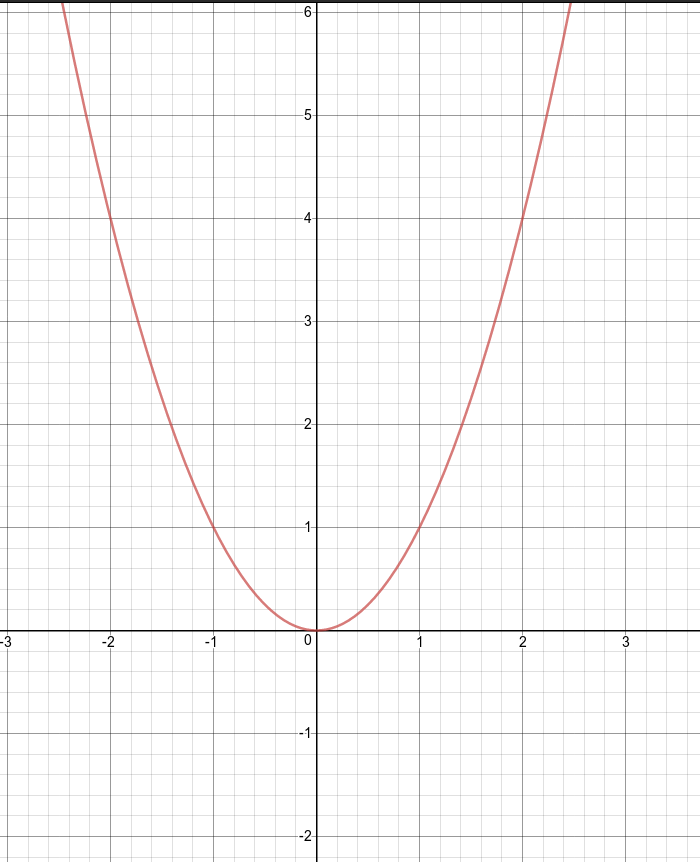
\includegraphics[scale=0.1]{parabola}

\begin{itemize}
\item Functions from $\R$ to $\R$ are usually given by formulas instead of
by drawing diagrams like in lesson 1.
\item For example let $f:\R\map\R$ be given by $f(x) = x^2$.
\item What is the $\dom(f)$?
\item Answer: $\R$.
\item What is the target set?
\item Answer $\R$.
\item What is $\ran(f)$.
\item Answer: $\setof{y\in\R}{y\geq 0}$.
\end{itemize}

\end{frame}

\begin{frame}{Functions from $\R to \R$}

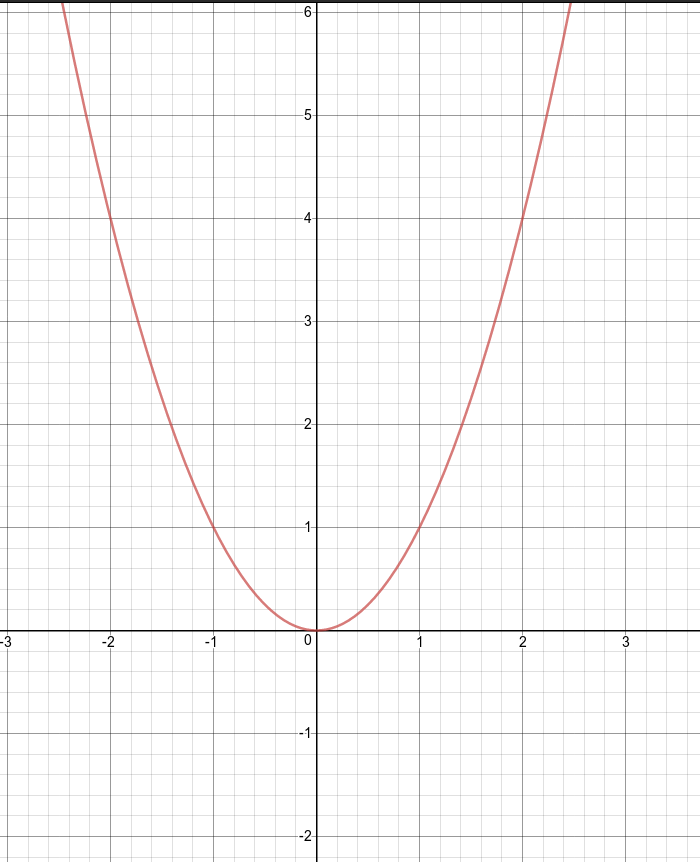
\includegraphics[scale=0.1]{parabola}

\begin{itemize}
\item Is $f$ one-to-one?
\item Answer: No, because, for example, $f(-1) = f(1)$.
\item Is $f$ onto?
\item Answer: No because the negative real numbers are not in the range.
\item What is $f\big[ [-2,2] \big]$?
\item Answer: $[0, 4]$
\end{itemize}

\end{frame}

\begin{frame}{Functions from $\R$ to $\R^2$}

\begin{itemize}
\item What does a function from $\R$ to $\R^2$ look like?
\item We need one input dimension but two output dimensions.
How do we represent this?
\item Also, how do we vizualize this? How do we graph it?
\item One common way to do this is as a \emph{parametric} plot:
\item $f(t) = (x(t), y(y))$
\end{itemize}

\end{frame}

\begin{frame}{Functions from $\R$ to $\R^2$}

\begin{columns}
\column[T]{5cm}
Let $A=[0, \infty)$. Let $f:A\map \R^2$ be defined by
$$f(t) = (t \cos(\pi t), t \sin(\pi t))$$
What does the graph of $f$ look like?
\column[T]{5cm}
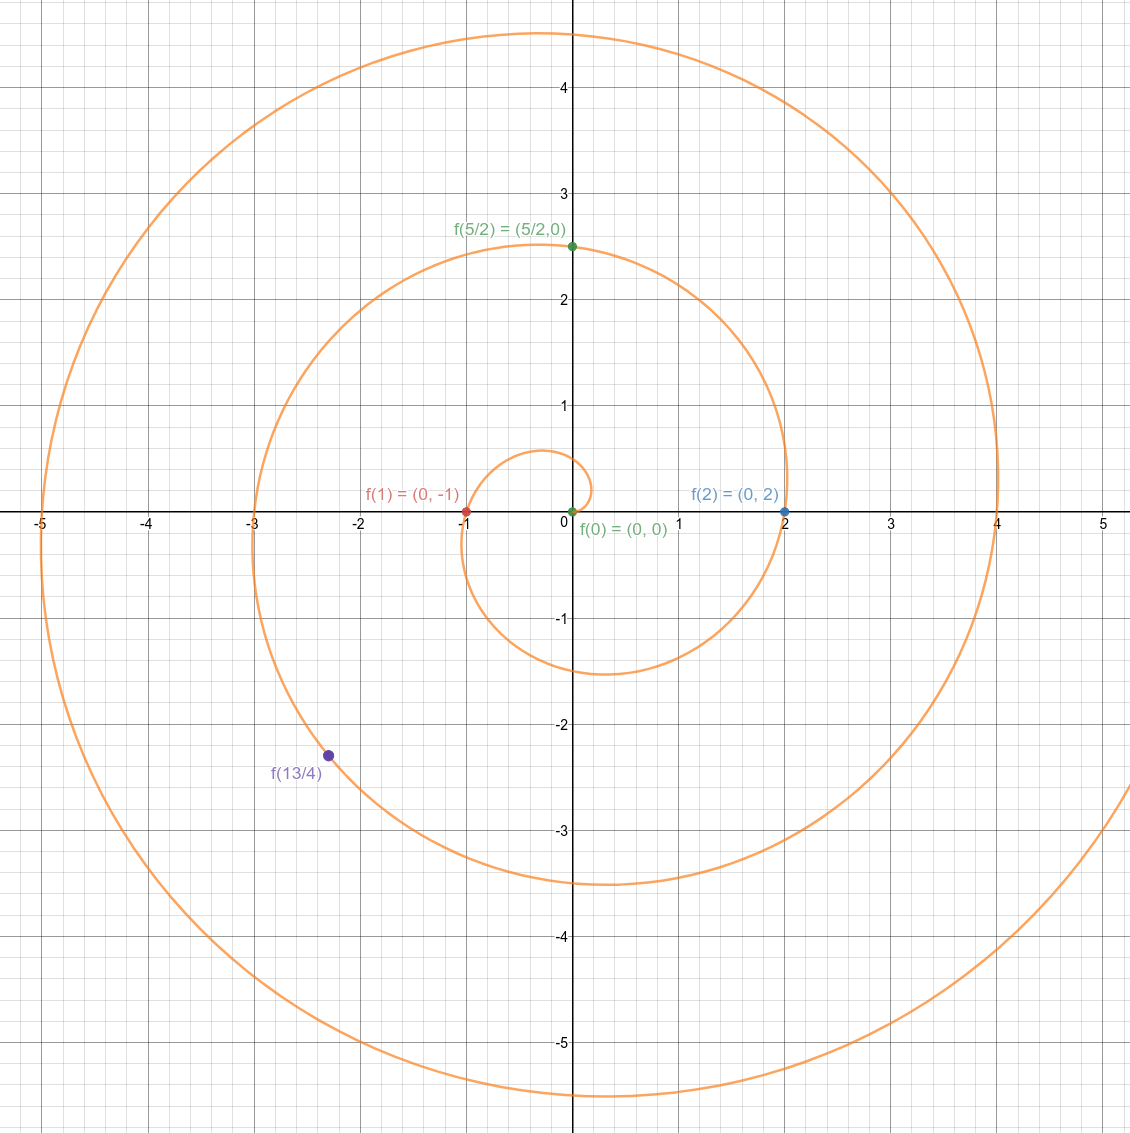
\includegraphics[scale=0.1]{spiral}
\end{columns}

\begin{itemize}
\item Is $f$ one-to-one?
\item Answer: Yes.
\item Is $f$ onto?
\item Answer: No
\item What are the domain, target and range of $f$?
\item $\dom(f) = A$, target is $\R^2$, range is the set of points on that
spiral.
\end{itemize}

\end{frame}

\begin{frame}{Functions from $\R$ to $\R^2$}

\begin{columns}
\column[T]{5cm}
Let $A=[0, \infty)$. Let $f:A\map \R^2$ be defined by
$$f(t) = (t \cos(\pi t), t \sin(\pi t))$$
\column[T]{5cm}
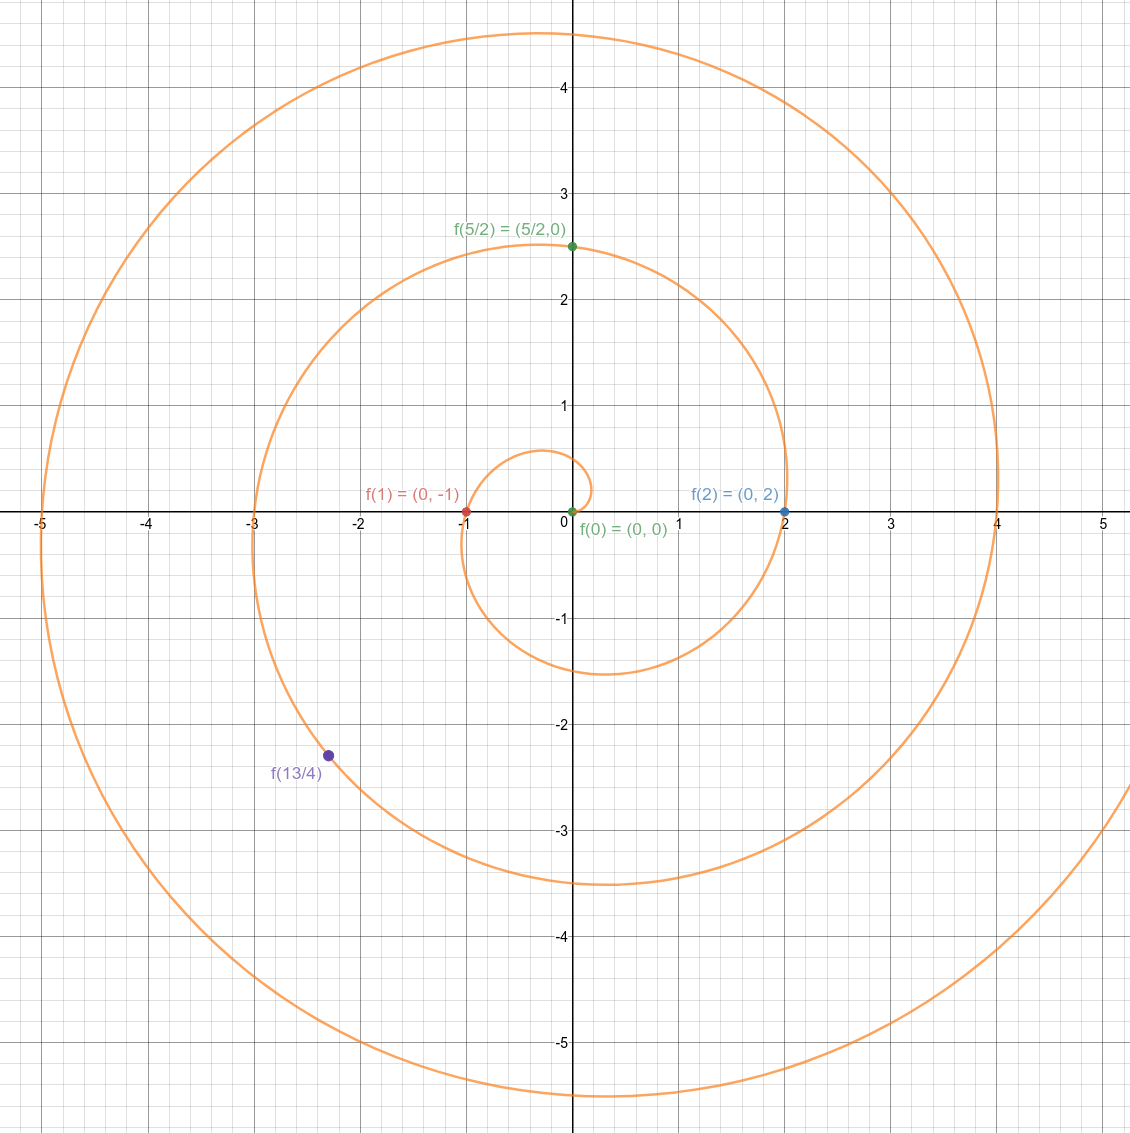
\includegraphics[scale=0.1]{spiral}
\end{columns}

\begin{itemize}
\item What is $f^{-1}[\singleton{(0,2)}]$?
\item Answer: $\singleton{2}$.
\item What is $f^{-1}[\singleton{(0,3)}]$?
\item Answer: $\emptyset$.
\end{itemize}

\end{frame}

\begin{frame}{Functions from $\R$ to $\R^2$}

\begin{columns}
\column[T]{5cm}
Let $A=[0, \infty)$. Let $f:A\map \R^2$ be defined by
$$f(t) = (t \cos(\pi t), t \sin(\pi t))$$
\column[T]{5cm}
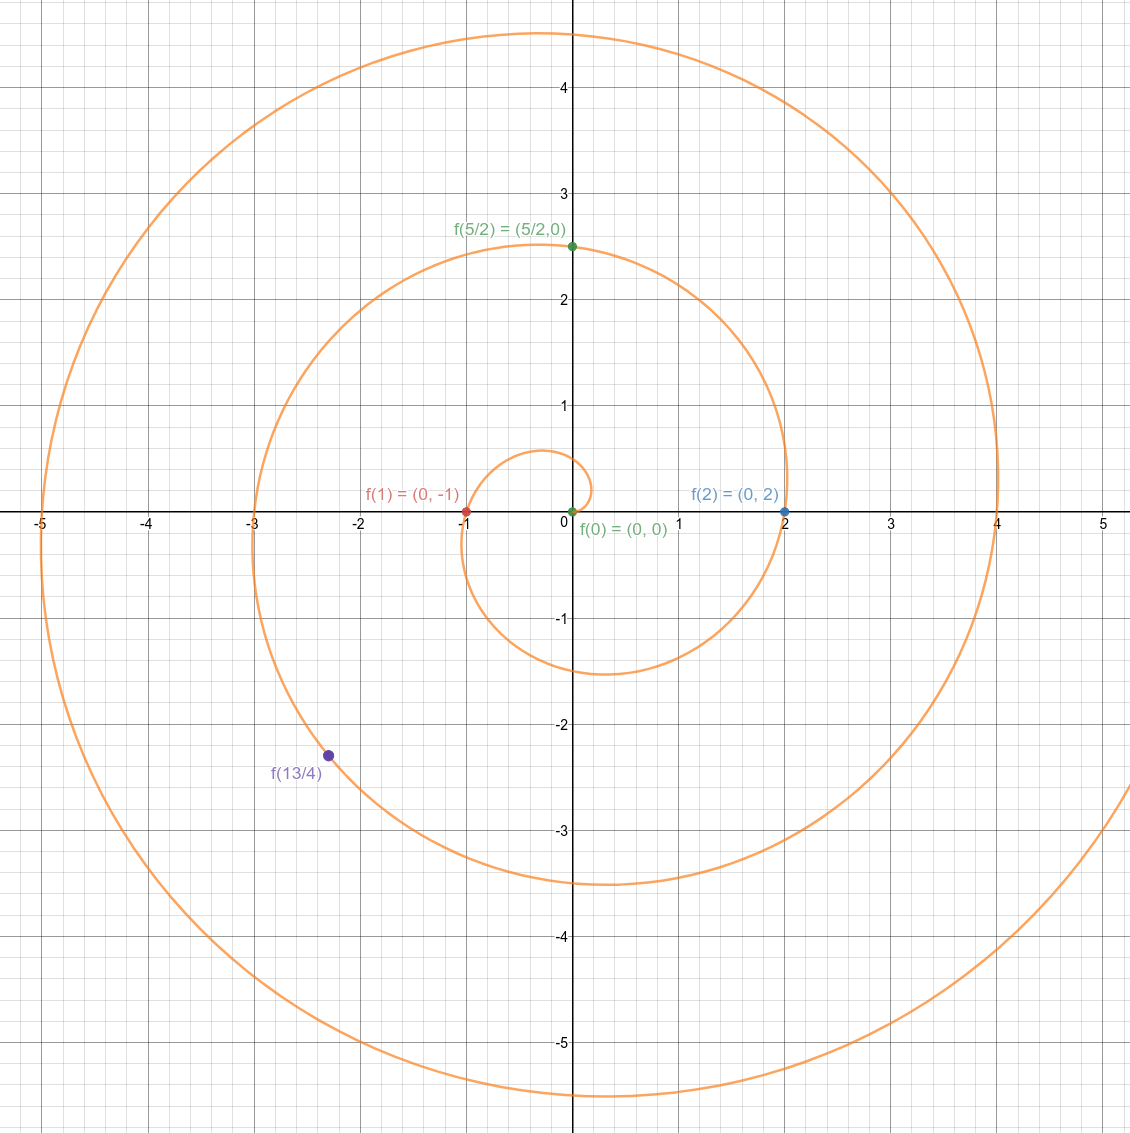
\includegraphics[scale=0.1]{spiral}
\end{columns}

\begin{itemize}
\item Question: What is the difference between the way we are \emph{picturing}
the function this time vs the way we pictured the function from
$\R$ to $\R$?
\item Answer: Here we are picturing \emph{only the target space} explicitly, not
the domain space. Previously we were picturing the domain space cross
the target space.
\end{itemize}

\end{frame}

\begin{frame}{Functions from $\R^2$ to $\R$}

\begin{itemize}
\item What does a function from $\R^2$ to $\R$ look like?
\item We need two input dimension but one output dimension.
How do we represent this?
\item Also, how do we vizualize this? How do we graph it?
\item $f(x,y) = z$
\item We can vizualize this as a surface over the $x$-, $y$- plane.
\item Then we are again picturing both the domain space and the target space
using their cross product.
\end{itemize}

\end{frame}

\begin{frame}{Functions from $\R^2$ to $\R$}

\begin{columns}
\column[T]{5cm}
Consider the function $f:\R^2\map\R$ given by
$$f(x,y) = x^2 + y$$
What does the graph of $f$ look like?
\column[T]{5cm}
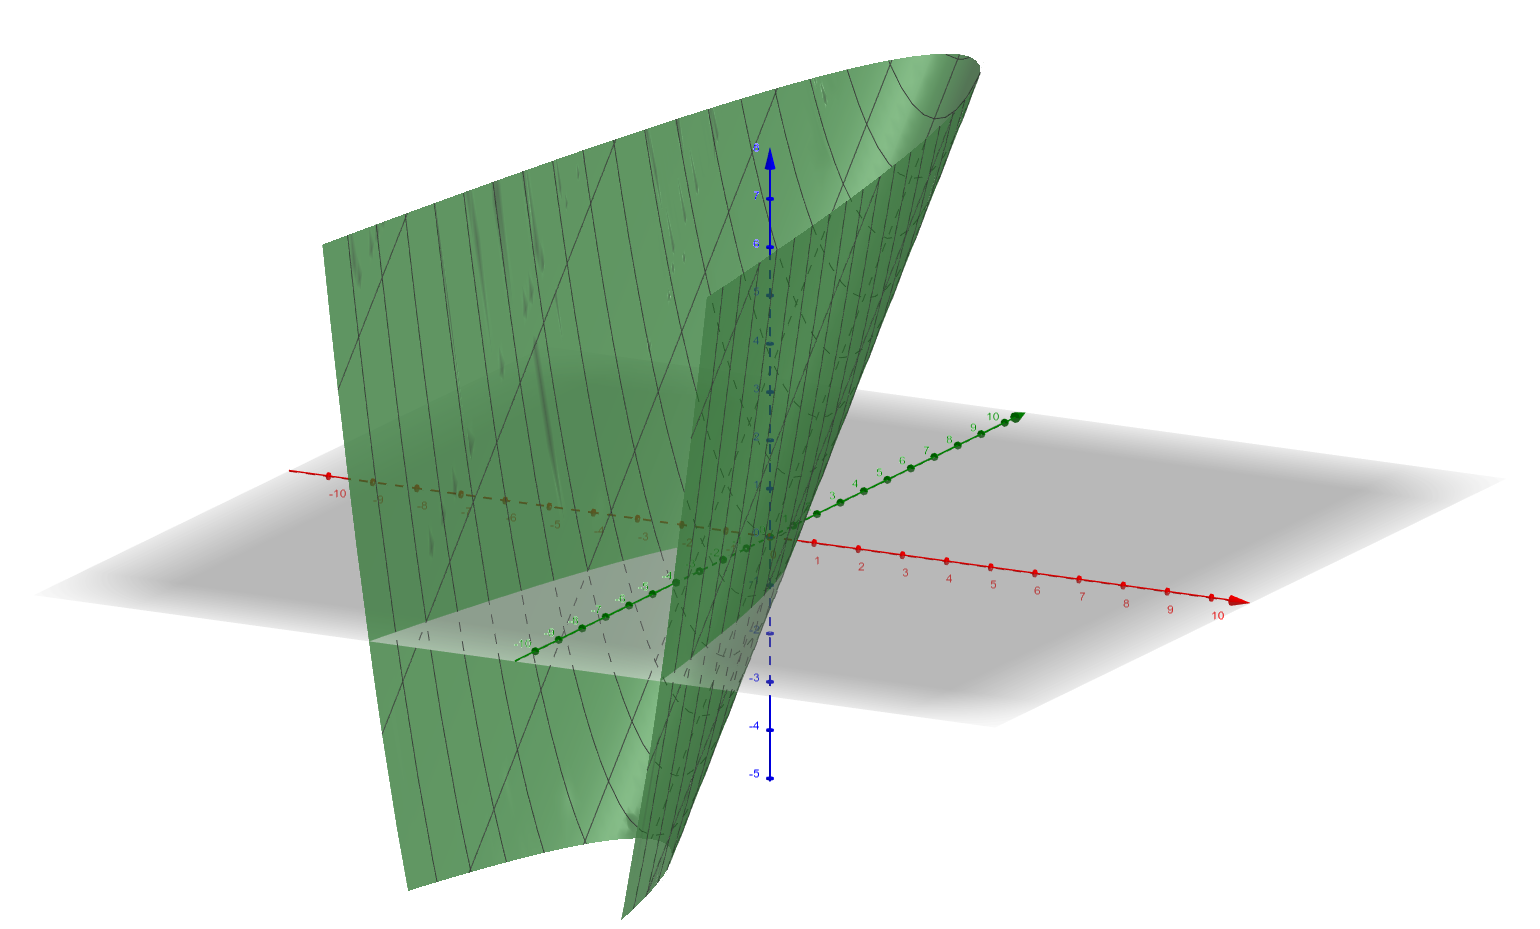
\includegraphics[scale=0.15]{x-squared-plus-y}
\end{columns}

\begin{itemize}
\item Is $f$ one-to-one?
\item No
\item Is $f$ onto?
\item Yes
\end{itemize}

\end{frame}

\begin{frame}{Functions from $\R^2$ to $\R$}


\begin{columns}
\column[T]{5cm}
\begin{itemize}
\item Another way to picture a function $f:\R^2\map\R$ is using
\emph{only the domain space}.
\item  We can draw the \emph{contour lines.}
\end{itemize}

Again consider the function $f:\R^2\map\R$ given by
$$f(x,y) = x^2 + y$$
\column[T]{5cm}
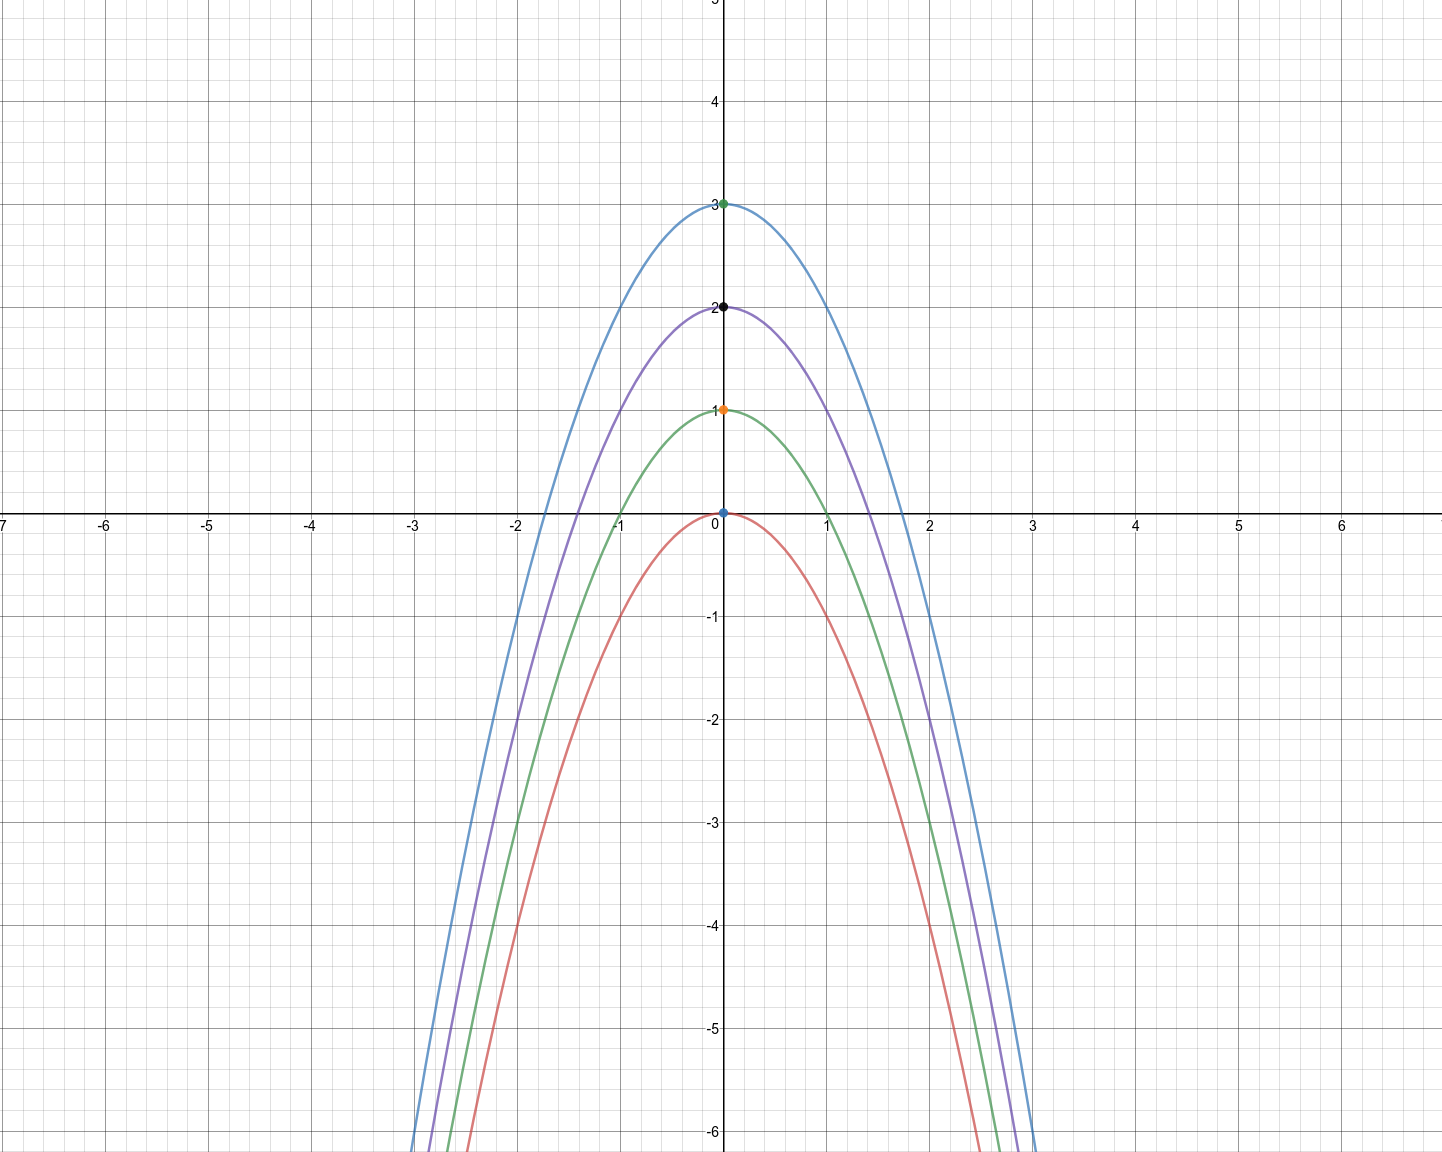
\includegraphics[scale=0.1]{contour-parabolas}
\end{columns}


\begin{itemize}
\item The parabolas are the inverse images of:
\item $\singleton{3}$
\item $\singleton{2}$
\item $\singleton{1}$
\item $\singleton{0}$
\end{itemize}
\end{frame}

\begin{frame}{Functions from $\R^2$ to $\R^2$}
\begin{itemize}
\item What does a function from $\R^2$ to $\R^2$ look like?
\item We need two input dimension and two output dimensions.
How do we represent this?
\item Also, how do we vizualize this? How do we picture it?
\item $f(x,y) = \big( u(x,y), v(x,y) \big)$
\item We cannot picture this using the cross-product of the domain space
and the target space because this is four dimensional.
\item One technique is we can picture a single $x$- $y$- plane to play
the role of both the domain and the target space and we can overlay
a region in the domain with its image in the target.
\end{itemize}
\end{frame}

\begin{frame}{Functions from $\R^2$ to $\R^2$}

\begin{columns}
\column[T]{5cm}
Consider
$$f(x,y) = (2x, y)$$

\begin{itemize}
\item $f(0, 0) = (0, 0)$
\item $f(1, 0) = (2, 0)$
\item $f(-1, 0) = (-2, 0)$
\item $f(0,1) = (0,1)$
\item $f(0,-1) = (0,-1)$
\end{itemize}

\column[T]{5cm}
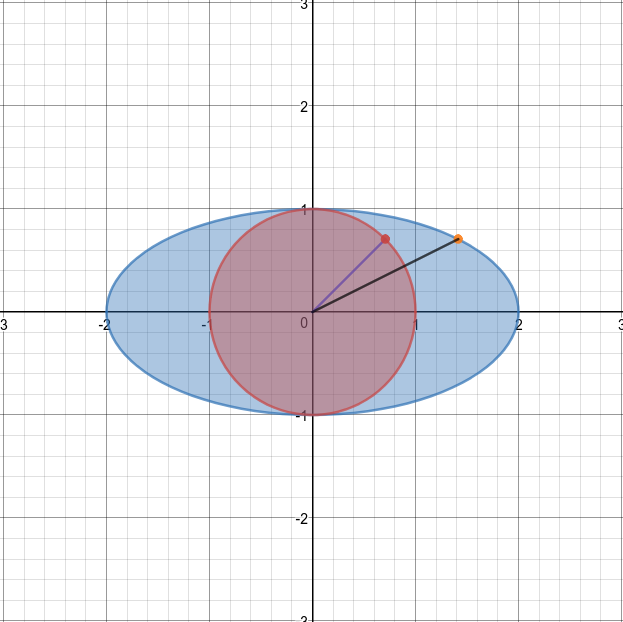
\includegraphics[scale=0.25]{circle-to-ellipse}
\end{columns}
\begin{itemize}
\item The image of the red circle is the blue ellipse
\item The image of the red point is the orange point.
\item The image of the purple line segment is the black line segment.
\end{itemize}

\end{frame}

\begin{frame}{Functions from $\R^2$ to $\R^2$}

\begin{columns}
\column[T]{5cm}
Consider
$$f(x,y) = (2x, y)$$

\column[T]{5cm}
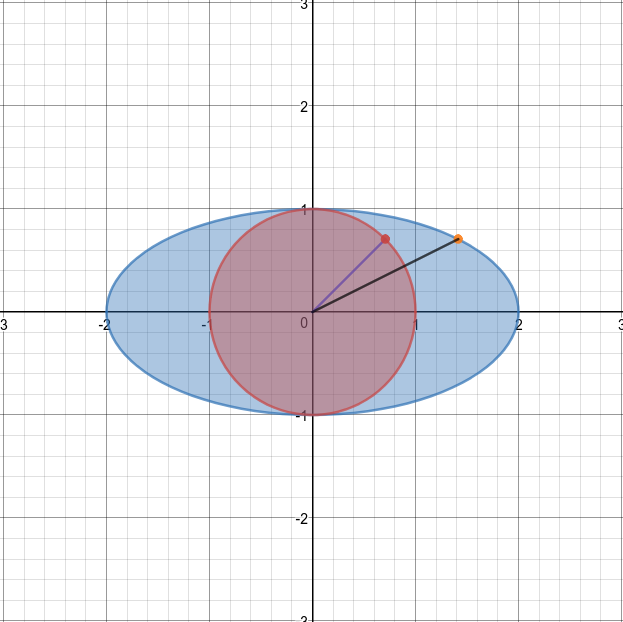
\includegraphics[scale=0.25]{circle-to-ellipse}
\end{columns}
\begin{itemize}
\item Is $f$ one-to-one?
\item Yes
\item Is $f$ onto?
\item Yes
\end{itemize}

\end{frame}

\begin{frame}{Functions from $\R^2$ to $\R^3$}
\begin{itemize}
\item What does a function from $\R^2$ to $\R^3$ look like?
\item We need two input dimension and three output dimensions.
How do we represent this?
\item Also, how do we vizualize this? How do we picture it?
\item $f(x,y) = \big( u(x,y), v(x,y), w(x,y) \big)$
\item We cannot picture this using the cross-product of the domain space
and the target space because this is five dimensional.
\item One technique is we can picture only the target space and think
of the function as parametric with two parameters.
\end{itemize}
\end{frame}

\begin{frame}{Functions from $\R^2$ to $\R^3$}

\begin{columns}
\column[T]{5cm}
Consider the function $f:\R^2\map\R^3$ given by
$$f(x,y) = (x , y, x^2 + y)$$
What does the graph of $f$ look like?
\column[T]{5cm}
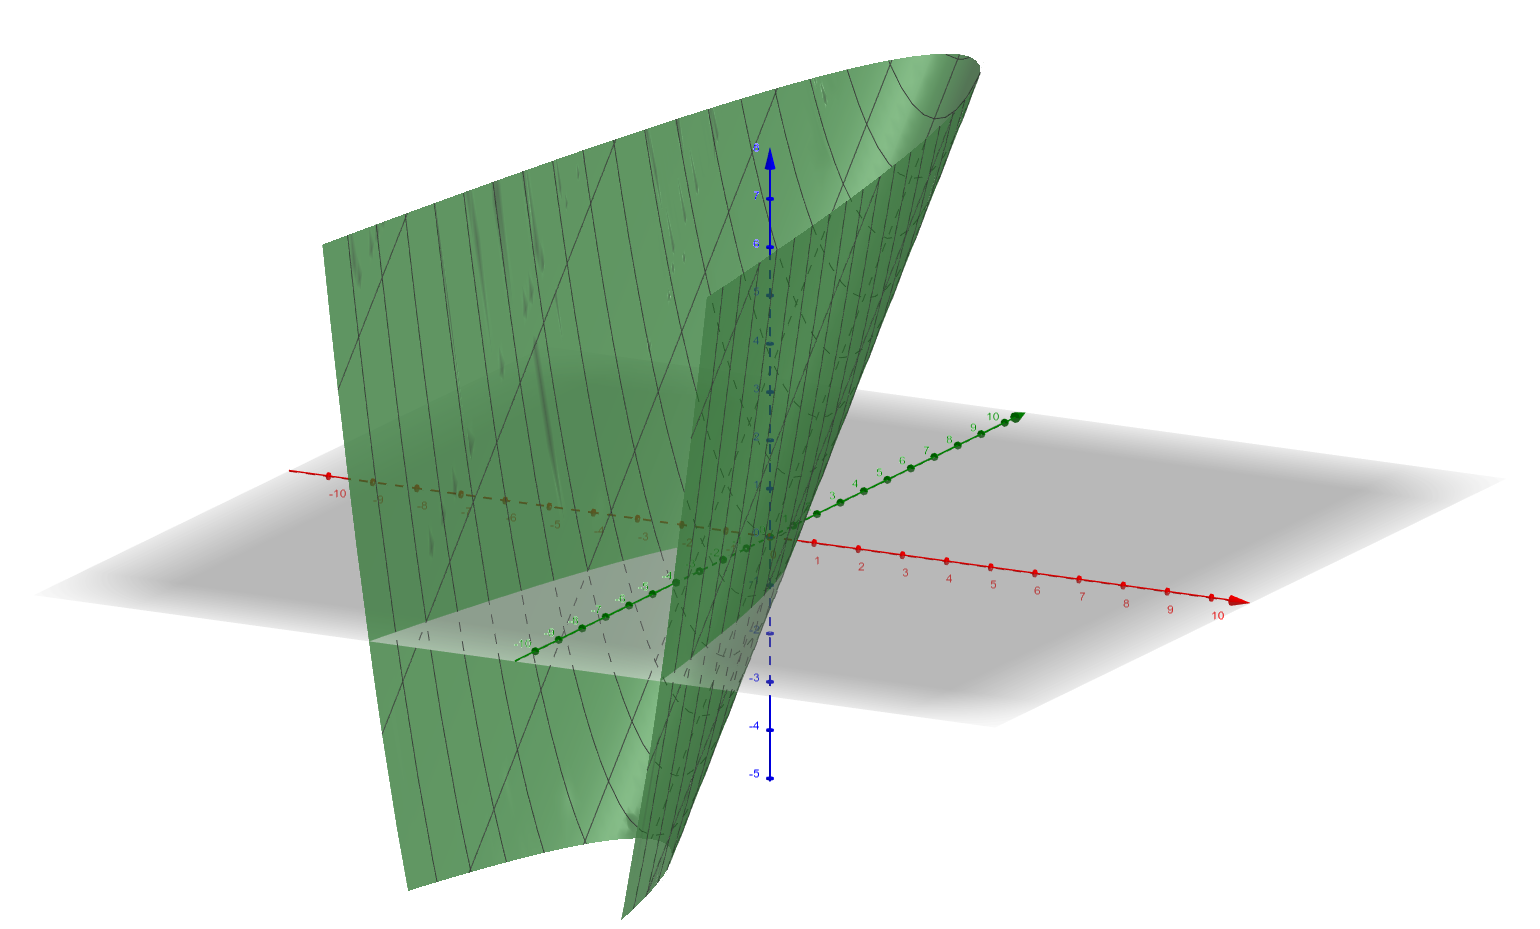
\includegraphics[scale=0.15]{x-squared-plus-y}
\end{columns}

\begin{itemize}
\item This is the same picture we used for a function from $\R^2$ to $\R$.
\item But now we are considering the picture to be of the target space
only instead of the domain space cross the target space.
\end{itemize}
\end{frame}

\begin{frame}{Functions from $\R^2$ to $\R^3$}

\begin{columns}
\column[T]{5cm}
$$f(x,y) = (x, y, x^2 + y)$$
\column[T]{5cm}
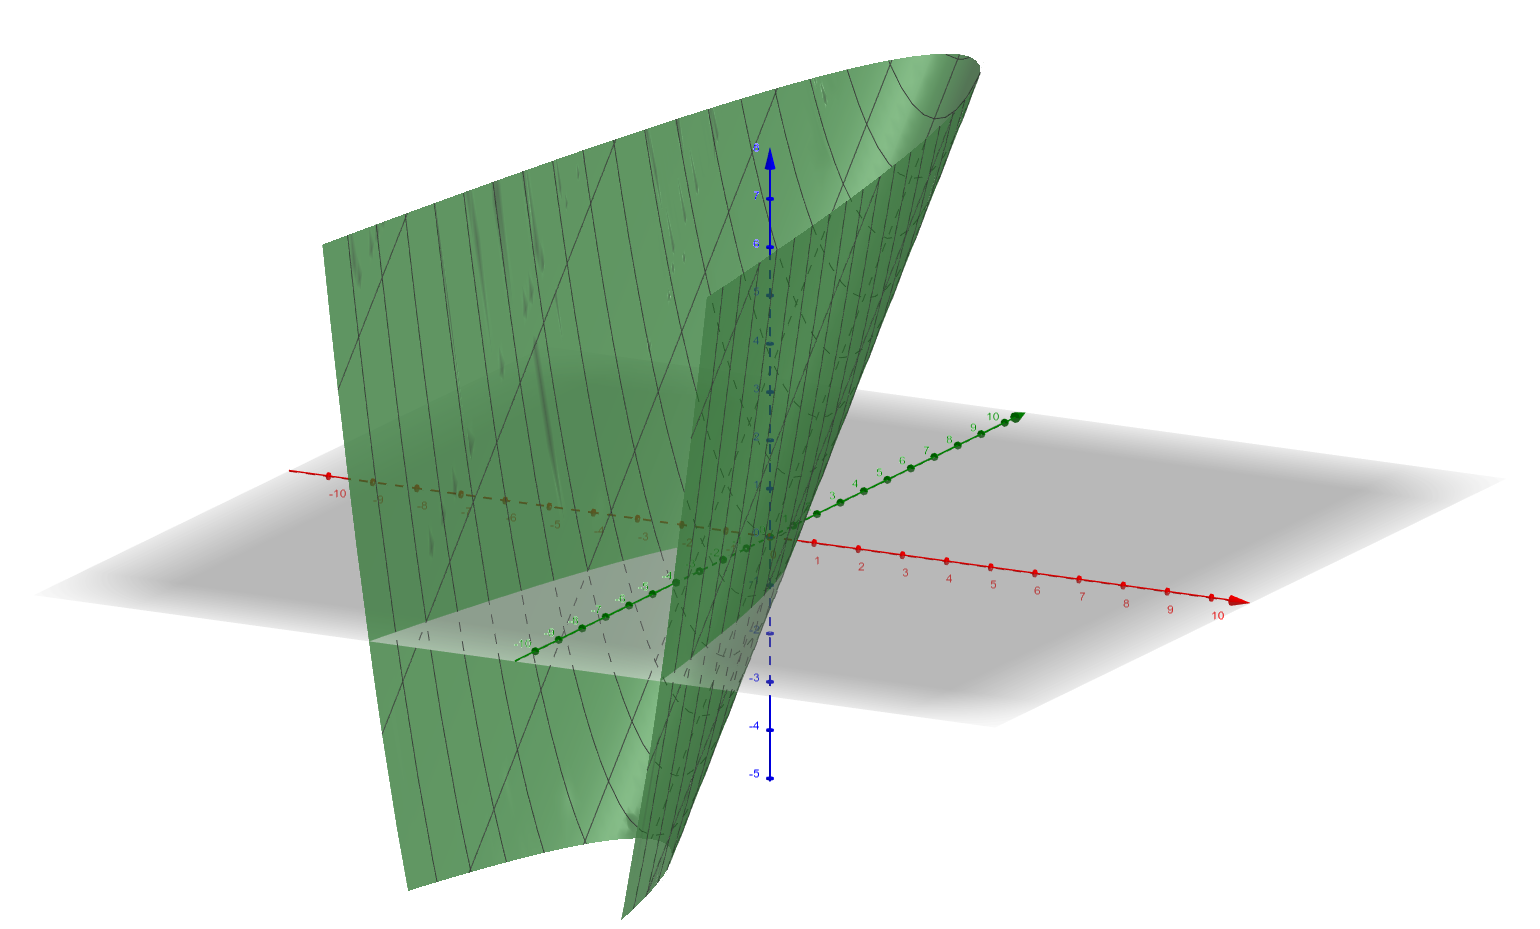
\includegraphics[scale=0.15]{x-squared-plus-y}
\end{columns}

\begin{itemize}
\item Is $f$ one-to-one?
\item Yes
\item Is $f$ onto?
\item No
\end{itemize}

\end{frame}


\begin{frame}{Functions from $\R^3$ to $\R^2$}

\begin{itemize}
\item What does a function from $\R^3$ to $\R^2$ look like?
\item We need three input dimension and two output dimensions.
How do we represent this?
\item Also, how do we vizualize this? How do we picture it?
\item $f(x,y,z) = \big( u(x,y,z), v(x,y,z) \big)$
\item We cannot picture this using the cross-product of the domain space
and the target space because this is five dimensional.
\item One technique is we can picture a single copy of $R^3$ and allow the
$x$-, $y$- plane to play two roles, both as part of the domain space and as
the target space.
\end{itemize}
\end{frame}

\begin{frame}{Functions from $\R^3$ to $\R^2$}

\begin{columns}
\column[T]{5cm}
Consider the function $f:\R^3\map\R^2$ given by
$$f(x,y, z) = \sqrt{\frac{x^2 + y^2 + z^2}{x^2+y^2}}(x, y)$$
$$f(0,0, z) = (0,0)$$
What does the graph of $f$ look like?
\column[T]{5cm}
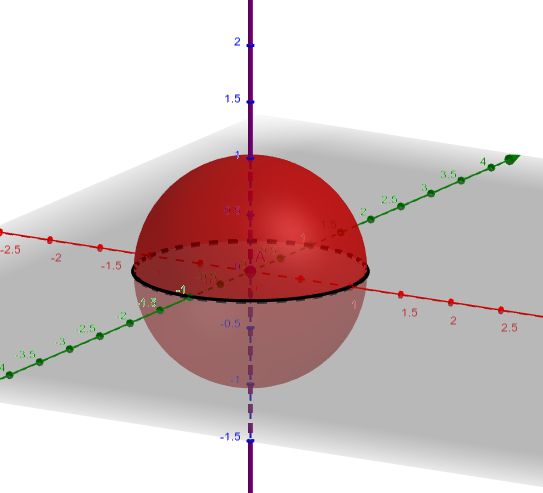
\includegraphics[scale=0.25]{sphere2}
\end{columns}

\begin{itemize}
\item The inverse image of the black circle is the red sphere of the same radius
minus the north and south poles.
\item What is $f^{-1}[\singleton{(0,0)}]$?
\item The $z$-axis
\end{itemize}
\end{frame}

\begin{frame}{Functions from $\R^3$ to $\R^2$}

\begin{columns}
\column[T]{5cm}
$$f(x,y, z) = \sqrt{\frac{x^2 + y^2 + z^2}{x^2+y^2}}(x, y)$$
$$f(0,0, z) = (0,0)$$
\column[T]{5cm}
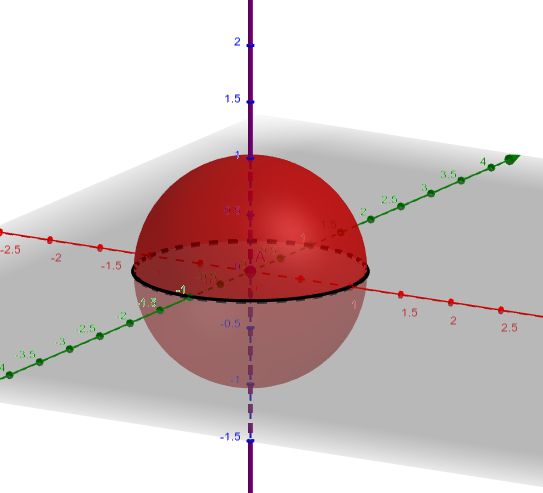
\includegraphics[scale=0.25]{sphere2}
\end{columns}

\begin{itemize}
\item Is $f$ one-to-one?
\item No
\item Is $f$ onto?
\item Yes
\end{itemize}
\end{frame}

\begin{frame}{Functions from $\R^3$ to $\R^3$}

\begin{itemize}
\item What does a function from $\R^3$ to $\R^3$ look like?
\item We need three input dimension and three output dimensions.
How do we represent this?
\item Also, how do we vizualize this? How do we picture it?
\item $f(x,y,z) = \big( u(x,y,z), v(x,y,z), w(x,y,z)\big)$
\item We cannot picture this using the cross-product of the domain space
and the target space because this is six dimensional.
\item One technique is we can picture a single copy of $\R^3$ to play
the role of both the domain and the target space and we can overlay
a region in the domain with its image in the target.
\end{itemize}
\end{frame}

\begin{frame}{Functions from $\R^3$ to $\R^3$}

\begin{columns}
\column[T]{5cm}
$$f(x,y, z) = (2x, y, z)$$
What is the image of the unit sphere?
\column[T]{5cm}
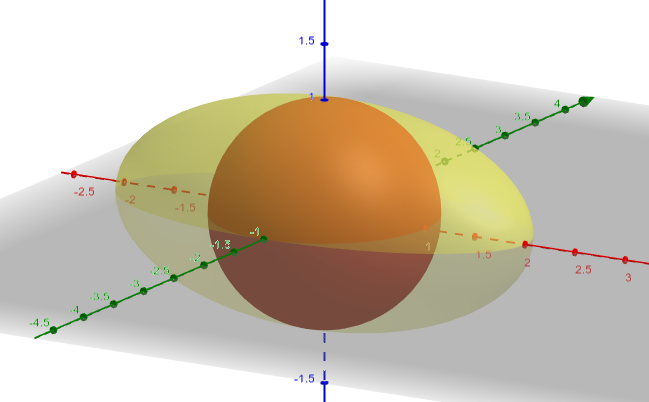
\includegraphics[scale=0.2]{sphere-to-ellipsoid}
\end{columns}

\begin{itemize}
\item Is $f$ one-to-one?
\item Yes
\item Is $f$ onto?
\item Yes
\end{itemize}
\end{frame}

\begin{frame}{Different ways of picturing functions from $\R^n$ to $\R^m$}


\begin{itemize}
\item Draw the entire \emph{graph} as a picture in $\R^n \times \R^m$
\item Draw a single copy of $\R^n$ to play the role of the domain space
and allow all or part of it to also play the role of the target space.
Overlay a region of the domain with its image.
\item Draw only the domain and picture a few inverse images.
\item Draw only the target and picture the range (parametric plot)
\end{itemize}

\end{frame}


\begin{frame}{Different ways of picturing functions from $\R^n$ to $\R^m$}


\begin{columns}
\column[T]{5cm}
\begin{itemize}
\item Draw the entire \emph{graph} as a picture in $\R^n \times \R^m$
\item $f:\R^1\map\R^1$ pictured in $\R^2$.
\item $f(x) = x^2$
\item $f:\R^2\map\R^1$ pictured in $\R^3$.
\item $f(x,y) = x^2 + y$
\end{itemize}

\column[T]{5cm}
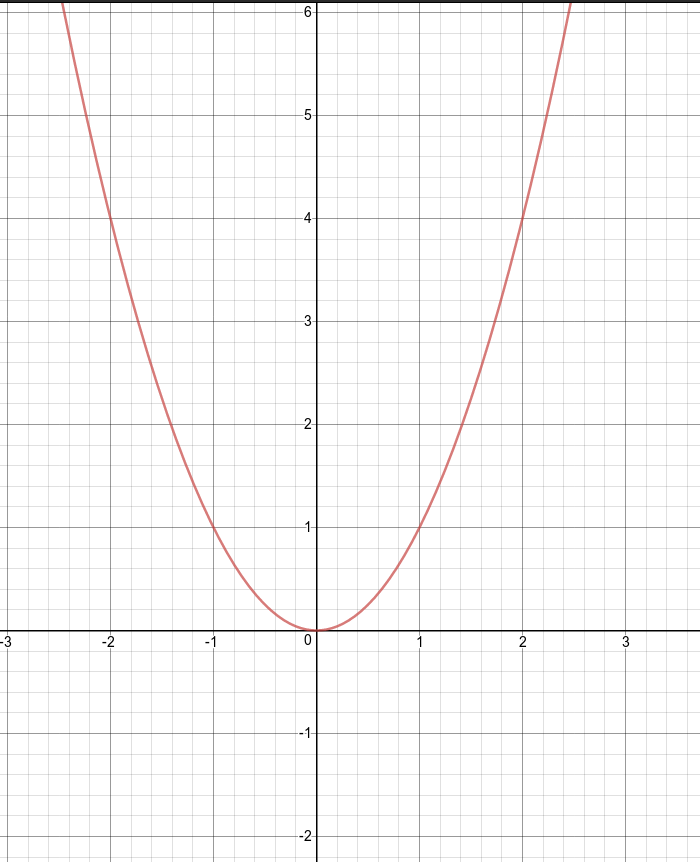
\includegraphics[scale=0.1]{parabola}

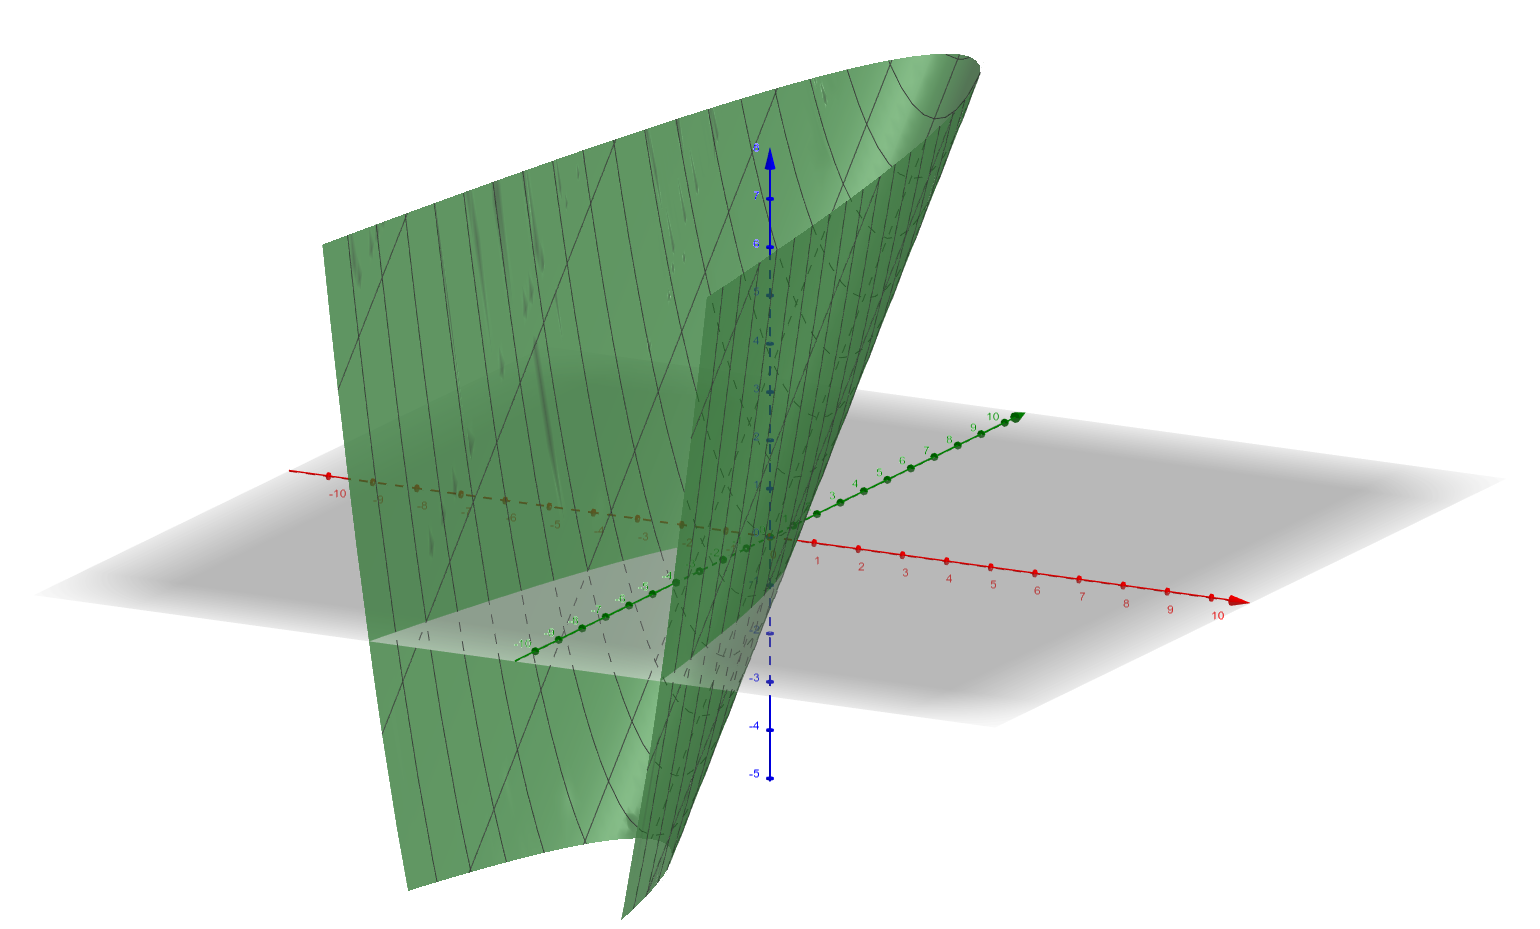
\includegraphics[scale=0.1]{x-squared-plus-y}
\end{columns}

\end{frame}

\begin{frame}{Different ways of picturing functions from $\R^n$ to $\R^m$}

\begin{columns}
\column[T]{5cm}
\begin{itemize}
\item Draw a single copy of $\R^n$ to play the role of the domain space
and allow all or part of it to also play the role of the target space.
\item $f:\R^2\map\R^2$ pictured in $\R^2$.
\item $f(x,y) = (2x, y)$
\item $f:\R^3\map\R^3$ pictured in $\R^3$.
\item $f(x,y, z) = (2x, y, z)$
\item $f:\R^3\map\R^2$ pictured in $\R^3$.
\end{itemize}

\column[T]{5cm}
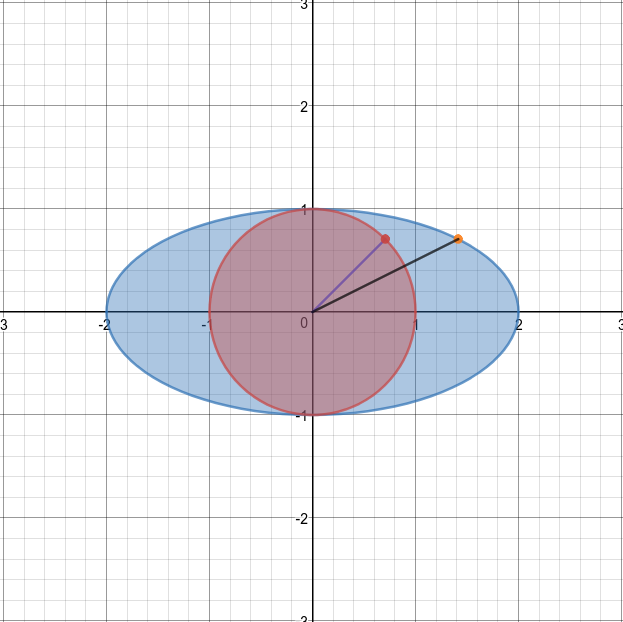
\includegraphics[scale=0.1]{circle-to-ellipse}

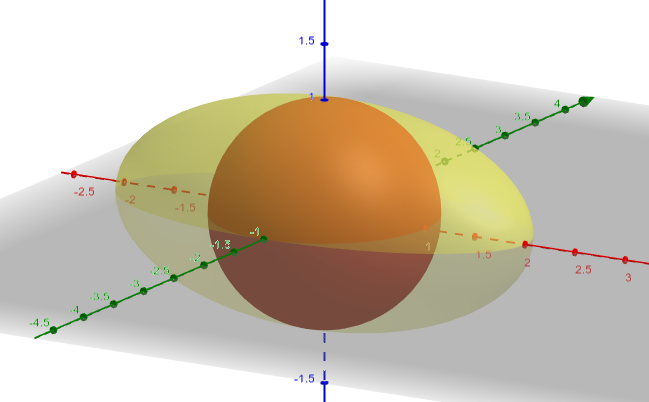
\includegraphics[scale=0.15]{sphere-to-ellipsoid}

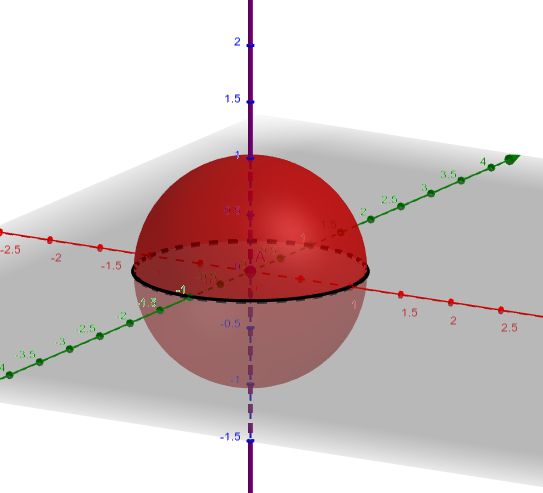
\includegraphics[scale=0.15]{sphere2}
\end{columns}

\end{frame}


\begin{frame}{Different ways of picturing functions from $\R^n$ to $\R^m$}

\begin{columns}
\column[T]{5cm}
\begin{itemize}
\item Draw only the domain and picture a few inverse images.
\item $f:\R^2\map\R^1$ pictured in $\R^2$.
\item $f(x,y) = x^2 + y$
\end{itemize}

\column[T]{5cm}
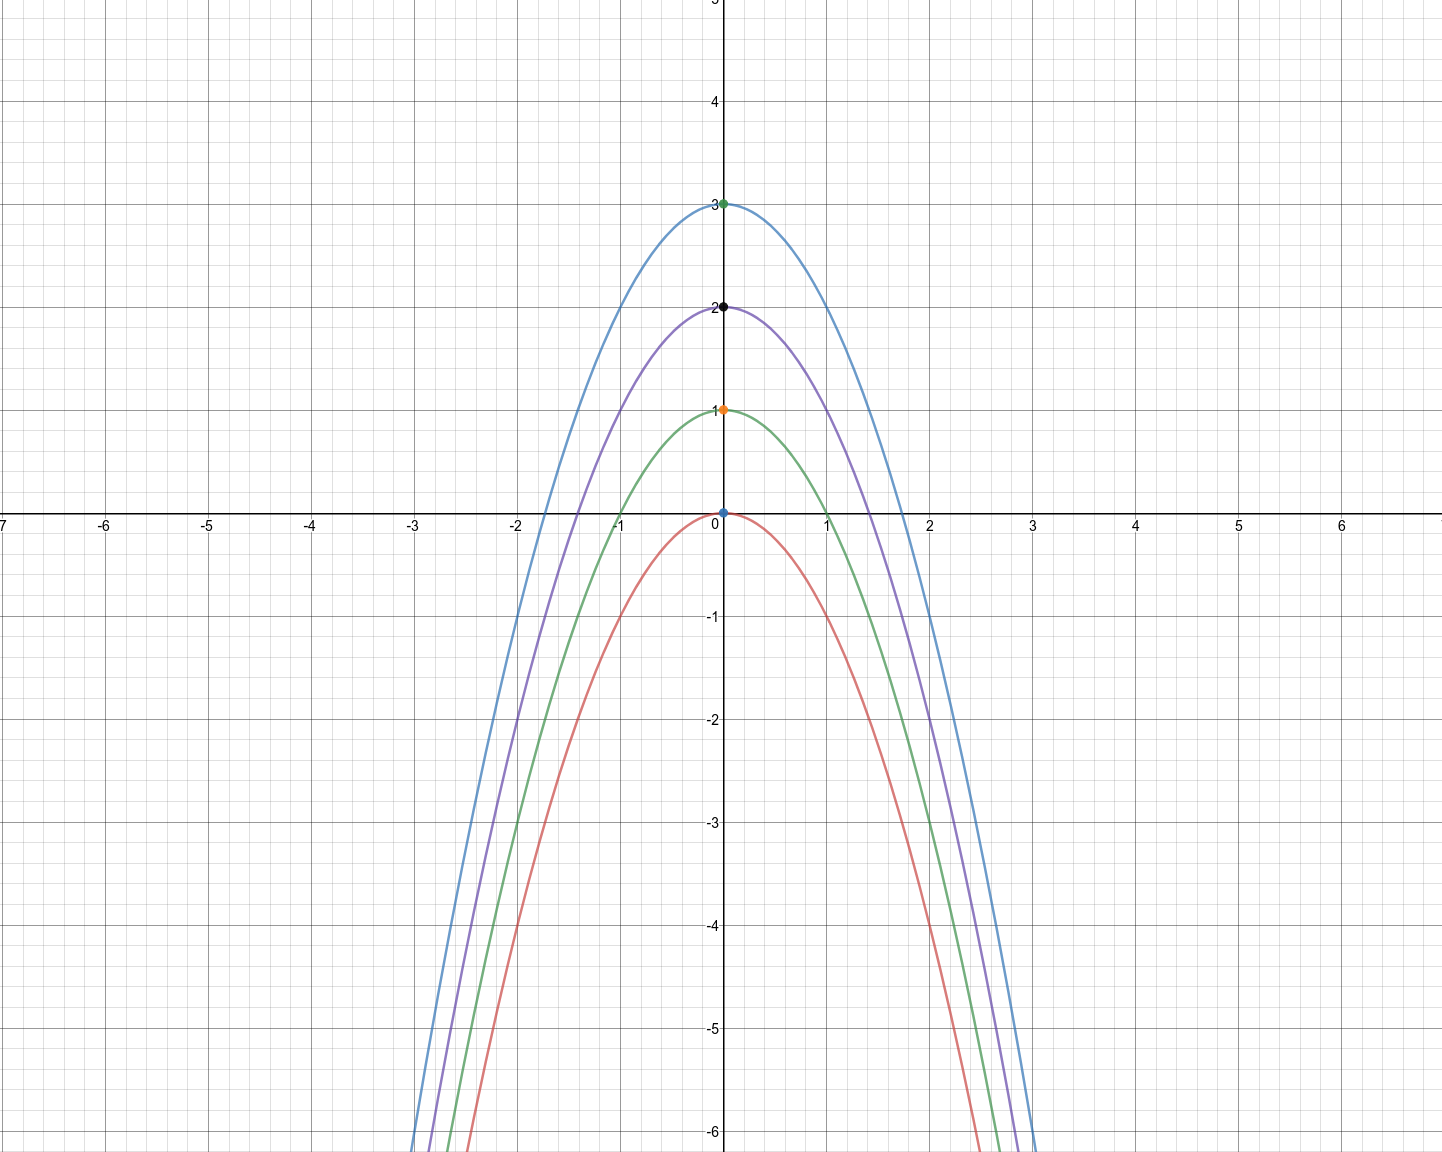
\includegraphics[scale=0.1]{contour-parabolas}

\end{columns}

\end{frame}

\begin{frame}{Different ways of picturing functions from $\R^n$ to $\R^m$}

\begin{columns}
\column[T]{5cm}
\begin{itemize}
\item Draw only the target and picture the range (parametric plot)
\item $f:\R\map\R^2$ pictured in $\R^2$.
\item $f(t) = (t \cos(\pi t), t \sin(\pi t))$
\item $f:\R^2\map\R^3$ pictured in $\R^3$.
\item $f(x,y) = (x , y, x^2 + y)$
\end{itemize}

\column[T]{5cm}
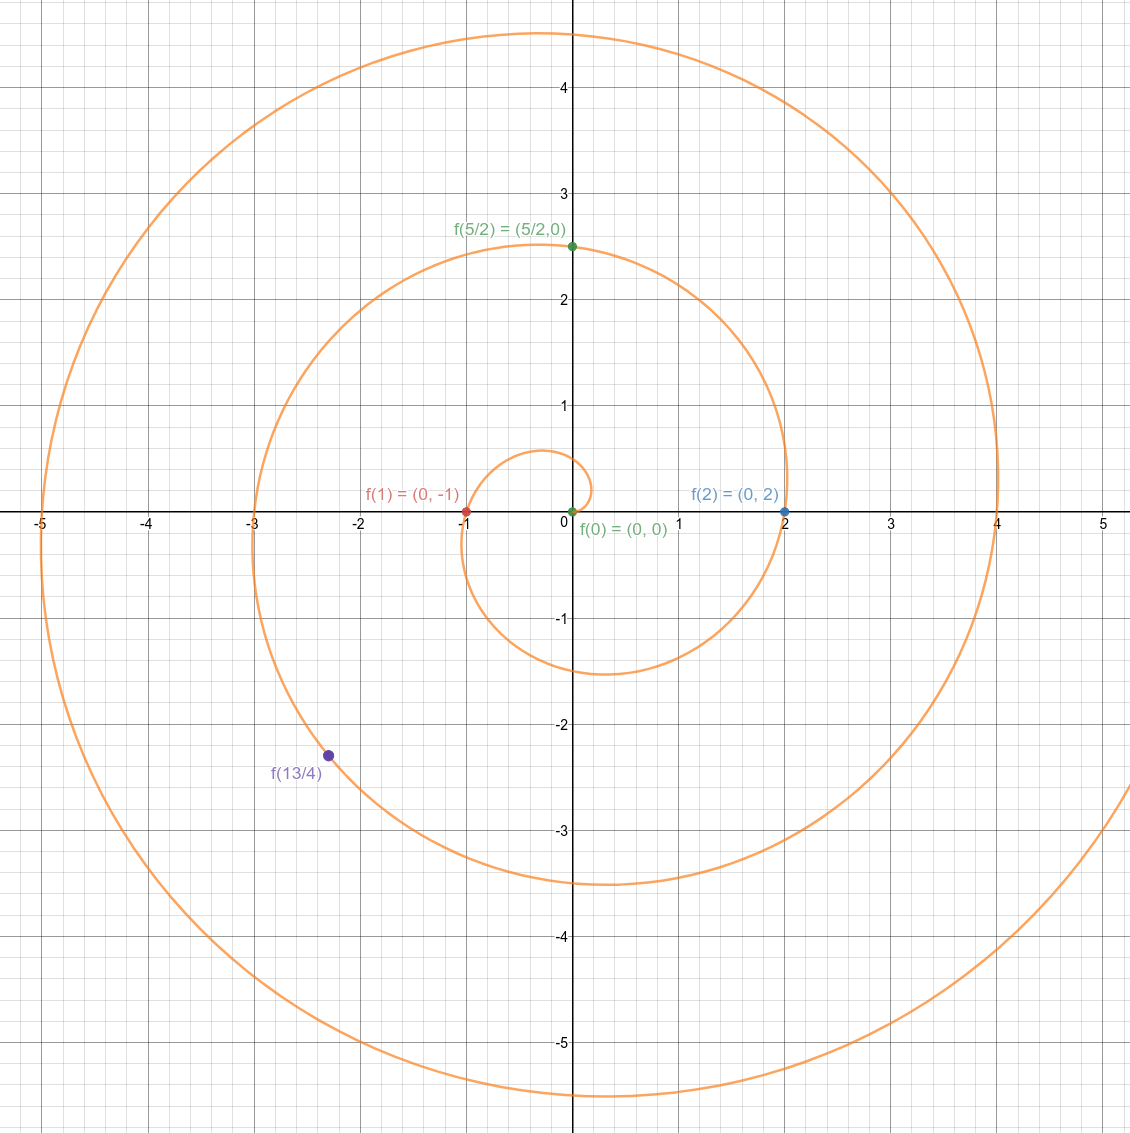
\includegraphics[scale=0.1]{spiral}

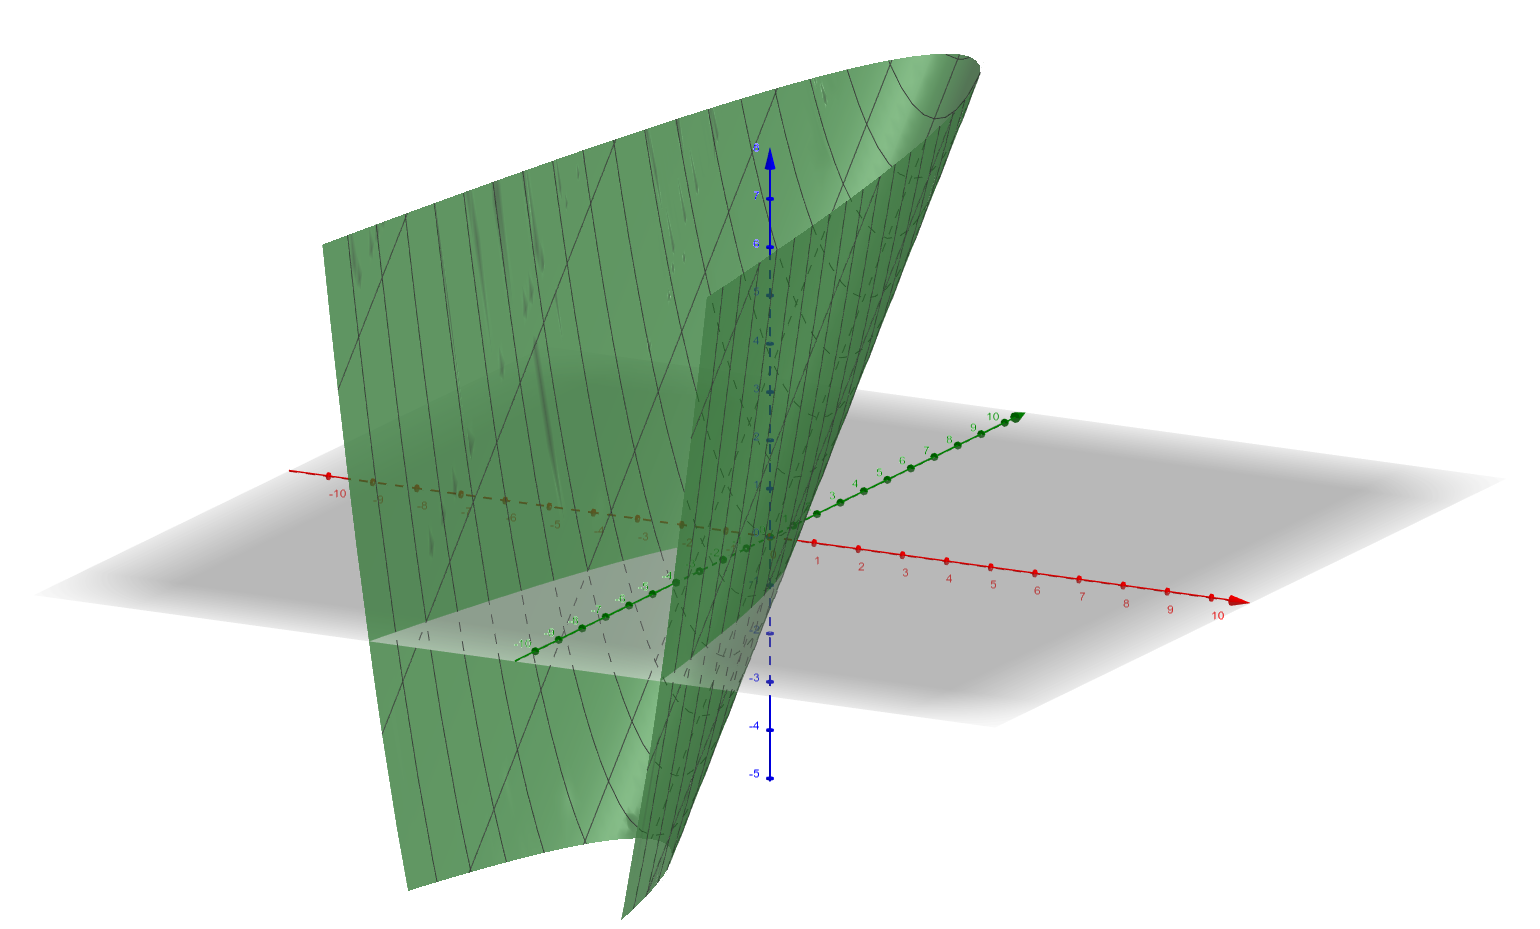
\includegraphics[scale=0.1]{x-squared-plus-y}

\end{columns}

\end{frame}



\end{document}

